\documentclass[a4paper, zihao=-4, UTF-8]{ctexart}
\usepackage{graphicx}
\usepackage{subfigure}
\usepackage{caption2}


\renewcommand{\figurename}{图}
\renewcommand{\captionlabeldelim}{.}
\renewcommand{\thesubfigure} {\thefigure.\arabic{subfigure}} \makeatletter
\renewcommand{\@thesubfigure}{\thesubfigure:\space} \renewcommand{\p@subfigure}{} \makeatother
\renewcommand{\tablename}{表}

\usepackage{enumerate}

\usepackage {ctex}
\usepackage{hyperref}
\hypersetup{
	colorlinks=true,
	citecolor=black,
	linkcolor=black
}

\usepackage{geometry}
\geometry{a4paper,left=2.5cm,right=2.5cm,top=2.5cm,bottom=2.5cm}
\setlength{\parindent}{2em}
\setmonofont{Consolas}
\setsansfont{Consolas}
\setmainfont{Times New Roman}

\usepackage{fancyhdr}
\pagestyle{fancy}
\renewcommand{\headrulewidth}{0pt}

\usepackage{authblk}
\renewcommand*{\Affilfont}{\small} % 修改机构名称的字体与大小
\renewcommand\Authand{, } % 去掉 and 前的逗号

\usepackage{indentfirst}
\setlength{\parindent}{2em}

\usepackage{amsmath}
\usepackage{amssymb}
\CTEXsetup[format={\Large\bfseries}]{section}
\usepackage{xcolor}
\usepackage{listings}
\renewcommand{\lstlistingname}{代码}
\lstset{
	columns=fixed,
	breakatwhitespace=true,
	breaklines=true,
	breakindent=26pt,
	captionpos=bl,
	numbers=left,
	frame=shadowbox,
	basicstyle=\ttfamily,
	keywordstyle=\ttfamily\color{blue},
	numberstyle=\footnotesize\color{darkgray},
	commentstyle=\ttfamily\it\color[RGB]{0,96,96},
	stringstyle=\ttfamily\color{magenta},
	showstringspaces=false,
	language=Python,
	identifierstyle=\ttfamily,
	tabsize=4,
}

\usepackage{algorithm}
\usepackage{algorithmicx}
\usepackage{algpseudocode}
\renewcommand{\algorithmicrequire}{\textbf{Input:}}  % Use Input in the format of Algorithm  
\renewcommand{\algorithmicensure}{\textbf{Output:}} % Use Output in the format of Algorithm  

\usepackage{appendix}
\renewcommand{\appendixname}{Appendix~\Alph{section}}
\usepackage{cleveref}
\crefname{equation}{式}{式}
\crefname{figure}{图}{图}
\crefname{table}{表}{表}
\crefname{appendix}{附录}{附录}
\crefname{algorithm}{算法}{算法}
\crefname{listing}{代码}{代码}
\newcommand{\crefpairconjunction}{~和~}
\newcommand{\crefmiddleconjunction}{、}
\newcommand{\creflastconjunction}{~和~}
\newcommand{\crefpairgroupconjunction}{~和~}
\newcommand{\crefmiddlegroupconjunction}{、}
\newcommand{\creflastgroupconjunction}{~和~}
\newcommand{\crefrangeconjunction}{~到~}

\usepackage{cite}
\newcommand{\upcite}[1]{{\textsuperscript{\cite{#1}}}}

\title{\textbf{密码学实验第五次实验报告} }
\date{}

\begin{document}
	\maketitle
	\tableofcontents
	\newpage
	\section{实验目的}
	\begin{enumerate}[1.]
		\item 通过本次实验,熟练掌握 AES-128 加解密流程;
		\item 了解 AES-192 与 AES-256 的加密流程;
		\item 了解 S 盒的生成原理;
		\item 通过尝试 AES 的攻击,了解常用的攻击方法。
	\end{enumerate}
	\section{实验原理}
	高级加密标准(Advanced Encryption Standard, AES)是美国联邦政府采用的一种分组加密标准。这个标准用来替代原先的 DES,已经被多方分析且广为全世界所使用。
	
	AES 的分组长度固定为 128bit,密钥长度则可以是 128,192 或者 256bit。根据密钥长度的不同,可将 AES 分为 AES-128,AES-192 和 AES-256。
	\section{实验环境}
		\paragraph*{系统环境} Windows10 WSL Ubuntu20.04。
		\paragraph*{运行环境} Python3.6与Python3.7。
	\section{实验内容}
	\subsection{算法原理}
	AES 算法使用了代换-置换网络结构(Substitution-Permutation Network, SPN),这种加密网络使用明文块和密钥块作为输入,并通过交错的若干轮代换操作和置换操作产生密文块。
	
	具体来说,AES 算法主要有四种操作处理,分别是轮密钥加(Add Round Key)、字节代替(SubByte)、行移位(Shift Rows)、列混淆(Mix Column)。明文和密钥都是由128bit 组成,以 Byte 为单位按照字节的先后顺序先从上到下、再从左到右进行排列。加密出的密文也按照相同顺序进行读取。AES 算法在处理的轮数上只有最后一轮操作与前面的轮处理上有些许不同,在轮处理开始前还单独进行了一次轮密钥加的处理。
	
	在密钥生成上,输入的密钥被扩展出 10 个轮密钥,每个轮密钥的长度均为 128bit,
	且两个轮密钥之间不存在重叠的字节。这些轮密钥也仅仅应用于轮密钥加中。
	\subsection{算法流程}
	\subsubsection{加密和解密}
	
	加密算法和解密算法的流程图如\cref{fig:crypt_flow_chart}所示。
	
	\begin{figure}[htbp]
		\centering
		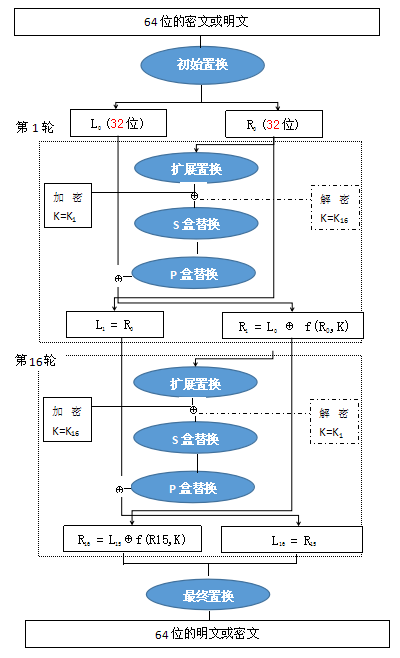
\includegraphics[width=\textwidth]{加解密流程图.png}
		\caption{加解密算法流程图}
		\label{fig:crypt_flow_chart}
	\end{figure}
	
	伪代码如\cref{alg:aes_encrypt}所示。解密时反向使用16个子密钥即可。
	\begin{algorithm}[htbp]
		\caption{加密和解密}
		\label{alg:aes_encrypt}
		\begin{algorithmic}[1]
			\Require 64位明文$input$,64位密钥$key$
			\Ensure 64位密文$output$
			\Function{AES\_Encrypt}{$input, key$}
			\State $K\gets \Call{KeyGen}{key}$;
			\State $state\gets input$;
			\State $\Call{AddRoundKey}{state, K[0,3]}$;
			\For{$round=1\to9$}
				\State $\Call{SubBytes}{state}$;
				\State $\Call{ShiftRows}{state}$;
				\State $\Call{MixColumns}{state}$;
				\State $\Call{AddRoundKey}{state, K[round \times 4, round \times 4 + 3]}$;
			\EndFor
			\State $\Call{SubBytes}{state}$;
			\State $\Call{ShiftRows}{state}$;
			\State $\Call{AddRoundKey}{state, K[40,43]}$;
			\State $output\gets state$;
			\State \Return{$K$}
			\EndFunction
		\end{algorithmic}
	\end{algorithm}
	\par 由上述流程图与代码对算法的描述可知,加密部分需要调用的函数有轮密钥加,字节代替,行移位和列混淆。
	\paragraph{轮密钥加} 在轮密钥加算法中,将 128 位的中间状态按位与 128 位的轮密钥进行异或运算。在这一步运算中,虽然运算方法简单,但由于密钥与中间状态等长,能够充分影响到每一位的结果。该函数伪代码如\cref{alg:addroundkey}所示。
	
	\begin{algorithm}[htbp]
		\caption{轮密钥加}
		\label{alg:addroundkey}
		\begin{algorithmic}[1]
			\Require $input[4][4]$,轮密钥$rk[4][4]$
			\Ensure $output[4]$
			\Function{AddRoundKey}{$input$, $table$}
			\State $state \gets input$;
			\For{$i=0\to 3$}
				\For{$j=0\to 3$}
					\State $state[i][j] \gets state[i][j]\oplus rk[i][j]$;
				\EndFor
			\EndFor
			\State $output\gets state$;
			\State \Return{$output$}
			\EndFunction
		\end{algorithmic}
	\end{algorithm}
	
	由于轮密钥加使用了异或运算,因此其逆变换是其本身,只需要使用相同的轮密钥进行计算即可。
	
	\paragraph{字节替换} AES 算法的字节替换函数,与 DES 算法中的 SBOX 较为相似,直接进行查表操作即可完成。其区别在于,AES 算法中的 SBOX 是由 $16\times16$ 个字节组成的矩阵,从中取数时,将高位作为行,低位作为列,以行列值为索引取数。伪代码如算法 3所示,其中,十六进制数字以 h 为结尾。
	
	\begin{algorithm}[htbp]
		\caption{字节替换}
		\label{alg:subbytes}
		\begin{algorithmic}[1]
			\Require $input[4][4], SBOX[256]$
			\Ensure $output[4][4]$
			\Function{SubBytes}{$input, SBOX$}
			\State $state\gets input$;
			\For{$i = 0\to 3$}
				\For{$j = 0 \to 3$}
					\State $state[i][j]=SBOX[state[i][j]]$;
				\EndFor
			\EndFor
			\State $output\gets state$;
			\State \Return{$output$}
			\EndFunction
		\end{algorithmic}
	\end{algorithm}
	
	SBOX的生成方式为:
	
	\begin{enumerate}[1.]
		\item 以索引值对 SBOX 进行初始化。
		\item 将每个字节映射到其在 $GF(2^8)$ 中的逆;对于 $0$ 则映射到其自身。
		\item 将每个字节的 8 位记为 $(b_7, b_6, b_5, b_4, b_3, b_2, b_1, b_0)$,进行如下矩阵运算:
			$$\left[\begin{matrix}
			1 & 0 & 0 & 0 & 1 & 1 & 1 & 1\\
			1 & 1 & 0 & 0 & 0 & 1 & 1 & 1\\
			1 & 1 & 1 & 0 & 0 & 0 & 1 & 1\\
			1 & 1 & 1 & 1 & 0 & 0 & 0 & 1\\
			1 & 1 & 1 & 1 & 1 & 0 & 0 & 0\\
			0 & 1 & 1 & 1 & 1 & 1 & 0 & 0\\
			0 & 0 & 1 & 1 & 1 & 1 & 1 & 0\\
			0 & 0 & 0 & 1 & 1 & 1 & 1 & 1
			\end{matrix}\right]\left[\begin{matrix}
			b_0 \\ b_1 \\ b_2 \\ b_3 \\ b_4 \\ b_5 \\ b_6 \\ b_7
			\end{matrix}\right]+\left[\begin{matrix}
			1 \\ 1 \\ 0 \\ 0 \\ 0 \\ 1 \\ 1 \\ 0
			\end{matrix}\right]=\left[\begin{matrix}
			b_0' \\ b_1' \\ b_2' \\ b_3' \\ b_4' \\ b_5' \\ b_6' \\ b_7'
			\end{matrix}\right]$$
		其结果为 SBOX 的值。需要注意的是,该矩阵运算中,所有的加法均为异或运算(即
		二元域上的加法)。
	\end{enumerate}
	
	在逆字节变换中,由于 SBOX 本身不可逆,因此需要为此构造另一个逆 SBOX,进行逆字节变换时,对逆 SBOX 进行查表即可。而对于逆 SBOX 的构造,可以直接对 SBOX求逆向的索引,也可以用数学方式进行求逆。数学方式如下:
	
	\begin{enumerate}
		\item 以索引值对逆 SBOX 进行初始化。
		\item 将每个字节记为 8 位,并进行如下矩阵运算:
		
		$$\left[\begin{matrix}
			0 & 0 & 1 & 0 & 0 & 1 & 0 & 1\\
			1 & 0 & 0 & 1 & 0 & 0 & 1 & 0\\
			0 & 1 & 0 & 0 & 1 & 0 & 0 & 1\\
			1 & 0 & 1 & 0 & 0 & 1 & 0 & 0\\
			0 & 1 & 0 & 1 & 0 & 0 & 1 & 0\\
			0 & 0 & 1 & 0 & 1 & 0 & 0 & 1\\
			1 & 0 & 0 & 1 & 0 & 1 & 0 & 0\\
			0 & 1 & 0 & 0 & 1 & 0 & 1 & 0\\
			\end{matrix}\right]\left[\begin{matrix}
			b_0 \\ b_1 \\ b_2 \\ b_3 \\ b_4 \\ b_5 \\ b_6 \\ b_7
			\end{matrix}\right]+\left[\begin{matrix}
			1 \\ 0 \\ 1 \\ 0 \\ 0 \\ 0 \\ 0 \\ 0
			\end{matrix}\right]=\left[\begin{matrix}
			b_0' \\ b_1' \\ b_2' \\ b_3' \\ b_4' \\ b_5' \\ b_6' \\ b_7'
		\end{matrix}\right]$$
		
		\item 将每个运算结果求 $GF(2^8)$ 上的逆,其结果就是逆 SBOX 的值。
	\end{enumerate}
	
	\paragraph{行移位} 行移位中,第一行保持不变,第二行向左循环移动一字节,第三行向左循环移动两字节,第四行向左循环移动三字节。逆行移位中,将所有左移变为右移即可。
	
	该函数的伪代码如\cref{alg:shiftrows}所示。
	
	\begin{algorithm}[htbp]
		\caption{行移位}
		\label{alg:shiftrows}
		\begin{algorithmic}[1]
			\Require $input[4]$
			\Ensure $output[4]$
			\Function{ShiftRows}{$input$}
			\For{$i=0\to 3$}
				\State $output[i]\gets (input[i] \gg i \times 8) \vee (input[i] \ll (3 − i) \times 8)$;
			\EndFor
			\State \Return{$output$}
			\EndFunction
		\end{algorithmic}
	\end{algorithm}

	行移位操作是 AES 几个操作中最简单的一个,但这个简单的操作在 AES 算法中却十分重要。通过移动位置,将每个字扩散到了整个状态当中,再配合列混淆等操作,使得每个字都能够很快地影响中间状态中的所有字,从而达到雪崩效应。
	
	\paragraph{列混淆} 列混淆是加解密过程中最复杂的部分,其目的也是用于扩散。列混淆混淆了输入矩阵的每一列,使每个输入的字节都会影响到当前一列的其他字节,行位移与列混淆的合并使用,使得每个字节在经过几轮过后都能影响到其它十六个字节,起到很好的扩散效果。列混淆的伪代码如\cref{alg:MixColumns}所示。
	
	\begin{algorithm}[htbp]
		\caption{密钥左旋}
		\label{alg:MixColumns}
		\begin{algorithmic}[1]
			\Require $input[4][4], columns\_matrix[4][4]$
			\Ensure $output[4][4]$
			\Function{MixColumns}{$input, columns\_matrix$}
			\State $output \gets \Call{MatrixMul}{columns\_matrix, input}$;
			\State \Return{$output$}
			\EndFunction
		\end{algorithmic}
	\end{algorithm}
	
	在列混淆中,需要给出一个 $4 \times 4$ 的矩阵,用这个矩阵右乘输入的矩阵,得到的结果便是这个函数的输出。而对于逆列混淆来说,只需要求出该 $4 \times 4$ 矩阵的逆,用这个逆矩阵再右乘加密后的矩阵,就能得到加密前的矩阵了。需要注意的是,在矩阵运算中,所有的数字均需要使用 $GF(2^8)$ 有限域上的加法和乘法。

	\subsubsection{轮密钥生成}
	轮密钥生成算法的整体流程图如\cref{fig:crypt_flow_chart}所示,对于每一轮来说,具体的生成算法流程示意图如\cref{fig:crypt_flow}所示。
	
	\begin{figure}[htbp]
		\centering
		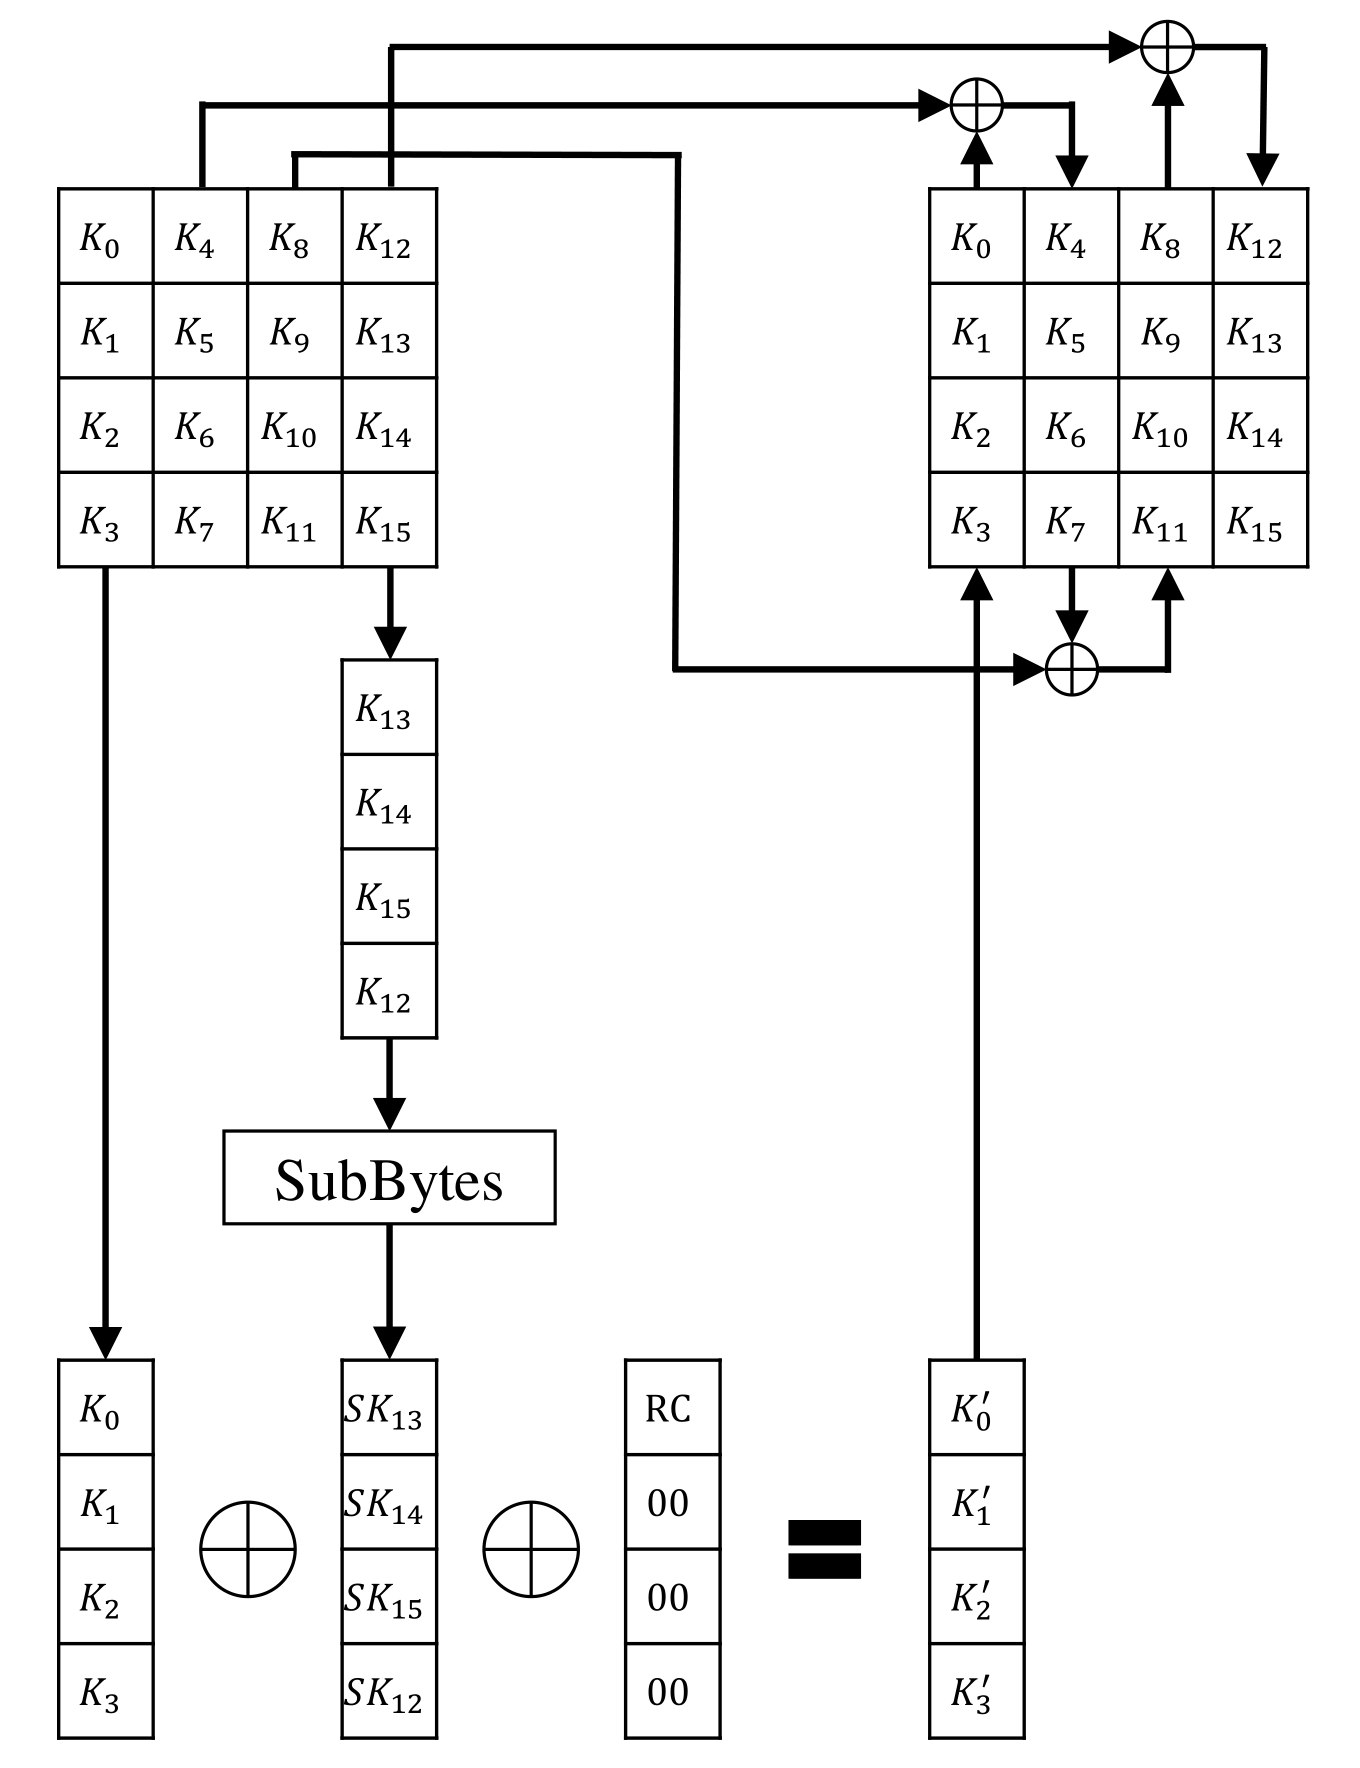
\includegraphics[width=\textwidth]{轮密钥生成算法流程图.png}
		\caption{轮密钥生成算法流程图}
		\label{fig:crypt_flow}
	\end{figure}
	
	伪代码如\cref{alg:keygen}所示。
	
	\begin{algorithm}[htbp]
		\caption{轮密钥生成}
		\label{alg:keygen}
		\begin{algorithmic}[1]
			\Require 128位密钥$key$
			\Ensure 轮密钥$K$
			\Function{KeyGen}{$key$}
			\For{$i=0\to3$}
				\State $K[i]\gets key[i \time 32, i\times 32 + 31]$;
			\EndFor
			\For{$i=1\to10$}
				\State $K[4\times i]\gets \Call{RotBytes}{K[4\times i - 1]}$;
				\State $K[4\times i]\gets \Call{SubBytes}{K[4\times i]}\oplus RC[i]$;
				\For{$j=0\to 3$}
					\State $K[4\times i + j]\gets K[4 \times i + j]\oplus K[4\times i + j - 4]$;
				\EndFor
			\EndFor
			\State \Return{$K$}
			\EndFunction
		\end{algorithmic}
	\end{algorithm}
	
	密钥扩展算法中,密钥将 128bit 输入拆分为 4 个字,每个字包含 32bit,输出则为44 个字的密钥和轮密钥,其中每四个为一个轮密钥,前四个字为初始密钥。加密算法中,每一次轮密钥加使用一个轮密钥,十一次轮密钥加与十一个轮密钥一一对应。
	
	对于其实现流程,大致如下:每个轮密钥仅由上一个轮密钥计算得出,且对于每一个字,仅由前四个字计算得出。每个轮密钥的第一个字中,需要使用包括字节替换,循环左移等函数进行更加复杂的变换,而对于其余的字,仅仅需要计算上一个字与前四个字的异或结果即可。
	由上述对算法的描述可知,轮密钥生成部分需要调用的函数为字节代替,其中字节左移部分实现较为简单,无需另写一个函数。由于字节代替部分与加解密中使用的函数完全相同,此处不再展开。
	
	\subsection{差分错误攻击}
	
	假设我们可以对加密过程中的倒数第二轮行移位运算后的某一个比特进行修改,并且我们知道这个修改发生的具体位置。在这个条件下,根据对后续运算的计算,以及错误密文与正确密文的偏差,可以有效缩小最后一轮轮密钥的可能取值。经过多次重复操作后,即可确定最后一轮的轮密钥。
	
	\subsubsection{分析过程} 现对标准 AES 进行分析。在经过第 9 轮的行移位后,注入一个错误(错误未知,而位置已知),不妨设错误发生在第一位,则有如下数学变换\upcite{1, 2}。
	
	$$F_{9,SR}=S_{9,SR}\oplus \left(\begin{matrix}
		\varepsilon & 0 & 0 & 0\\
		0 & 0 & 0 & 0\\
		0 & 0 & 0 & 0\\
		0 & 0 & 0 & 0\\
	\end{matrix}\right)$$
	
	其中,$F_{N,XX}$ 为注入错误后的错误矩阵,$S_{N,XX}$ 为正确矩阵,下标表示第 $N$ 轮经过 $XX$变换后的矩阵。
	
	经过列混淆后
	
	$$F_{9,MC}=S_{9,MC}\oplus \left(\begin{matrix}
		2\cdot\varepsilon & 0 & 0 & 0\\
		\varepsilon & 0 & 0 & 0\\
		\varepsilon & 0 & 0 & 0\\
		3\cdot\varepsilon & 0 & 0 & 0\\
	\end{matrix}\right)$$
	
	轮密钥加后
	
	$$F_{9,ARK}=S_{9,ARK}\oplus \left(\begin{matrix}
		2\cdot\varepsilon & 0 & 0 & 0\\
		\varepsilon & 0 & 0 & 0\\
		\varepsilon & 0 & 0 & 0\\
		3\cdot\varepsilon & 0 & 0 & 0\\
	\end{matrix}\right)$$
	
	第十轮的字节替换后,设替换后的值分别为 $\varepsilon_0', \varepsilon_1', \varepsilon_2', \varepsilon_3'$
	
	$$F_{10,SB}=S_{10,SB}\oplus \left(\begin{matrix}
		\varepsilon_0' & 0 & 0 & 0\\
		\varepsilon_1' & 0 & 0 & 0\\
		\varepsilon_2' & 0 & 0 & 0\\
		\varepsilon_3' & 0 & 0 & 0\\
	\end{matrix}\right)$$
	
	行移位后
	
	$$F_{10,SR}=S_{10,SR}\oplus \left(\begin{matrix}
		\varepsilon_0' & 0 & 0 & 0\\
		0 & 0 & 0 & \varepsilon_1'\\
		0 & 0 & \varepsilon_2' & 0\\
		0 & \varepsilon_3' & 0 & 0\\
	\end{matrix}\right)$$
	
	经过最后的轮密钥加后,得到最终的错误密文
	
	$$F_{10,ARK}=S_{10,ARK}\oplus \left(\begin{matrix}
		\varepsilon_0' & 0 & 0 & 0\\
		0 & 0 & 0 & \varepsilon_1'\\
		0 & 0 & \varepsilon_2' & 0\\
		0 & \varepsilon_3' & 0 & 0\\
	\end{matrix}\right)$$
	
	由该结果可以得到一组等式:
	
	$$\begin{cases}
		s(x_0+2\varepsilon)=s(x_0)+\varepsilon_0'\\
		s(x_1+\ \varepsilon)=s(x_1)+\varepsilon_1'\\
		s(x_2+\ \varepsilon)=s(x_2)+\varepsilon_2'\\
		s(x_3+3\varepsilon)=s(x_3)+\varepsilon_3'\\
	\end{cases}$$
	
	总的来说,错误注入攻击的原理就是根据 AES 最后一轮混淆与置换不彻底的性质,一个字节的变化仅仅影响了结果中的四个字节,可以从中获取出一系列等式关系,从而缩小密钥空间。
	
	\subsubsection{错误注入}
	
	在得到上述等式组后,显然 $\varepsilon$ 和 $x_i$ 的取值范围均在 $0$ 到 $\mathrm{0x}100$ 之间,可以分别对等式 $s(x_i + c\varepsilon) = s(x_i) + \varepsilon_i'$ 进行爆破,将其得到的集合进行相交即可得到所有可能的初始错误注入 $\varepsilon$ 的值。
	
	随后得到所有 $\varepsilon$ 的可能取值后,根据等式关系对所有可能进行尝试,可以分别得到每个位置在进行错误注入前的值 $x$。
	
	根据正确计算时的等式 $s(x)\oplus key = CA$,$CA$ 表示正确结果,即可得到该位置密钥的所有可能取值。
	
	将如上步骤重复多次后,将结果进行集合的交运算,可以完全确定某四位末轮密钥。随后只需移动错误注入的位置,并继续重复以上操作,即可确定全部十六比特的末轮密钥。由末轮密钥进行密钥生成算法的反向计算,即可计算得到初始密钥。
	
	其伪代码如\cref{alg:differentialfault}所示。
	
	\begin{algorithm}[htbp]
		\caption{错误注入}
		\label{alg:differentialfault}
		\begin{algorithmic}[1]
			\Require $\varepsilon'[4], c[4], CA[4]$
			\Ensure $K[4]$
			\Function{DifferentialFaultAnalysis}{$\varepsilon'[4],c[4]$}
			\For{$i=0\to3$}
			\State $K[i]\gets key[i \time 32, i\times 32 + 31]$;
			\EndFor
			\For{$i=1\to10$}
			\State $K[4\times i]\gets \Call{RotBytes}{K[4\times i - 1]}$;
			\State $K[4\times i]\gets \Call{SubBytes}{K[4\times i]}\oplus RC[i]$;
			\For{$j=0\to 3$}
			\State $K[4\times i + j]\gets K[4 \times i + j]\oplus K[4\times i + j - 4]$;
			\EndFor
			\EndFor
			\State \Return{$K$}
			\EndFunction
		\end{algorithmic}
	\end{algorithm}
	
	在错误注入的具体实现中,为模拟第九轮特定位置被注入的场景,攻击函数调用了第九轮后的几个加密函数。为此,需要向攻击函数提供注入前的结果,以及仅为模拟加密机准备的第九轮与第十轮密钥,而不参与到实际的破解中。
	
	\subsection{测试样例与结果截图}
	测试样例如\cref{apx:testdata}中的\cref{lst:aestestdata}所示。
	\par 结果截图如\cref{fig:aestestres}所示。
	\begin{figure}[htbp]
		\centering
		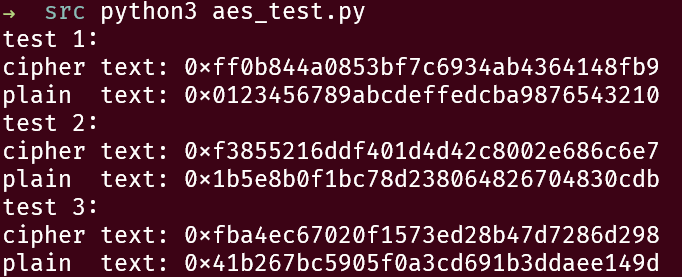
\includegraphics{aes_test_res.png}
		\caption{AES算法测试数据结果截图}
		\label{fig:aestestres}
	\end{figure}
	
	错误注入攻击结果如\cref{fig:aestestattack}所示。
	
	\begin{figure}[htbp]
		\centering
		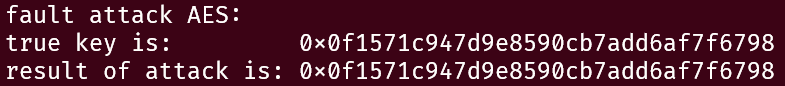
\includegraphics{错误注入攻击.png}
		\caption{AES算法错误注入测试结果截图}
		\label{fig:aestestattack}
	\end{figure}
	\section{收获与建议}
	\paragraph{收获} 在 AES 代码的书写中,考虑到命名空间的问题,选择在无需向外部提供调用的函数名称前添加下划线,可以将其变为私有函数,有效避免命名空间冲突的问题,并且能够缩短函数名称长度,提高代码的可阅读性。
	
	在错误注入中,需要对文献中为展示的位置进行注入,此时可能对等式的 $c$ 值进行错误的调用。此时需要仿照文献中的计算步骤,对具体的运算后的结果进行判断。经过具体运算后发现,若错误注入的位置在第一行,则 $c$ 值均为 $\{2, 1, 1, 3\}$。同理,若错误在第 $i$ 行,则 $c$ 值为列混淆矩阵的第 $i$ 列。行移位部分则较为容易分析出,此处不再赘述。
	
	由于提供的参考文献写得较为简略,实现时可以同时参考其引用的原始文献,如文献\upcite{1} 中包含了测试数据,可以在编写程序时辅助查找代码中的细节问题。
	
	差分错误分析对于大部分分组密码来说都较为有效,其原因在于分组算法的混淆与扩散依赖于多轮运算,一旦在最后一轮中可以被注入错误,该错误的混淆与扩散效果较差,且混淆与扩散的结果可以成功用于破解最后一轮的密钥。然而,这种攻击方式具有较大的局限性,实际应用中,攻击者需要可以向缓存中注入错误才可以实现。因此,分组密码的整体结构仍然具有较高的安全性。
	
	\paragraph{建议} 本次实验中,个人认为选做题在一般难度与困难难度两道题上难度差距较大,而简单难度与一般难度之间的差距较小,希望后续实验中对难度梯度的设计更加合理。
	\begin{thebibliography}{99}
		\bibitem{1}
		Giraud C. (2005) DFA on AES. In: Dobbertin H., Rijmen V., Sowa A. (eds) Advanced		Encryption Standard –AES. AES 2004. Lecture Notes in Computer Science, vol 3373.		Springer, Berlin, Heidelberg. https://doi.org/10.1007/11506447\_4
		\bibitem{2}
		孙维东, 俞军, 沈磊. 对称加密算法 AES 和 DES 的差分错误分析 [J]. 复旦学报 (自然		科学版),2013,52(03):297-302.
	\end{thebibliography}
	\newpage
	\appendix
	
	\section{思考题}
	\subsection{比较AES与DES的异同}
	AES 与 DES 两个加密算法都是分组密码算法,都需要先对数据分块再进行加密,并且在密钥的使用上,都需要对将一个密钥扩展为多个轮密钥,再应用到相应的轮函数中。
	
	两个算法的区别主要体现在具体的设计上。在使用的原理上,DES 算法使用了 Feistel密码结构,而 AES 算法使用了 SPN 结构;在初始划分中,DES 将数据分为左右两部分,AES 则将数据转化为一个 4 × 4 的矩阵,对整个矩阵进行加密;在明文大小和密钥大小上,DES 使用了 64 位明文和 56 位密文,标准的 AES 使用了 128 位明文和 128 位密文;在具体的轮次上,DES 计算了 16 轮,标准的 AES 计算了 10 轮。
	
	从 AES 与 DES 的区别中可以看出,由于 AES 有着更大的密钥空间,且加密时混淆更加彻底,其安全性更强,而由于其加密轮次较少,因此速度反而更快。
	\section{测试样例}\label{apx:testdata}
	\begin{lstlisting}[caption={AES测试样例}, label={lst:aestestdata}]
aes_test = [
	[0x123456789abcdeffedcba9876543210, 0x0f1571c947d9e8590cb7add6af7f6798], 
	[0x1b5e8b0f1bc78d238064826704830cdb, 0x3475bd76fa040b73f521ffcd9de93f24], 
	[0x41b267bc5905f0a3cd691b3ddaee149d, 0x2b24424b9fed596659842a4d0b007c61]
]
i = 1
for test in aes_test:
	print (f'test {i}: ')
	i += 1
	cipher = CNSPP.aes_encrypt(test[0], test[1])
	print ('cipher text: ', end = '')
	CNSPP.print_hex_as_len(cipher, 32)
	print ('plain  text: ', end = '')
	CNSPP.print_hex_as_len(CNSPP.aes_decrypt(cipher, test[1]), 32)

print ('fault attack AES: ')
print ('true key is:         0x0f1571c947d9e8590cb7add6af7f6798')
print ('result of attack is: ', end = '')
key_9 = [
	[ 0xfd, 0x0e, 0xc5, 0xf9 ],
	[ 0x0d, 0x16, 0xd5, 0x6b ],
	[ 0x42, 0xe0, 0x4a, 0x41 ],
	[ 0xcb, 0x1c, 0x6e, 0x56 ]
]

key_10 = [
	[ 0xb4, 0xba, 0x7f, 0x86 ],
	[ 0x8e, 0x98, 0x4d, 0x26 ],
	[ 0xf3, 0x13, 0x59, 0x18 ],
	[ 0x52, 0x4e, 0x20, 0x76 ],
]

array_to_inject = [
	[ 0x99, 0x1e, 0x73, 0xf1 ],
	[ 0x18, 0x15, 0x30, 0xaf ],
	[ 0x97, 0x3b, 0x84, 0xdd ],
	[ 0xa7, 0x08, 0x08, 0x0c ],
]
CNSPP.print_hex_as_len(CNSPP.error_injection(array_to_inject, key_9, key_10), 32)
	\end{lstlisting}
	
\end{document}